\section{The case of oriented knot diagrams}

\subsection{Labeling homomorphism with orientation}

Every knot diagram can be endowed with orientation in two different ways. Given an oriented knot diagram there are two distinct types of crossings as seen in \cref{fig:4:two:types:crossings}. In such crossings segments $i$ and $o$ are easily distinguishable, allowing us to write two different elements to which labeling homomorphism $\phi$ will map segments that contribute to one crossing:
$$+:\phi(u,i,o)=au+bi+co$$
$$-:\phi(u,i,o)=\alpha u+\beta i+\gamma o.$$

\begin{figure}[h]\centering
  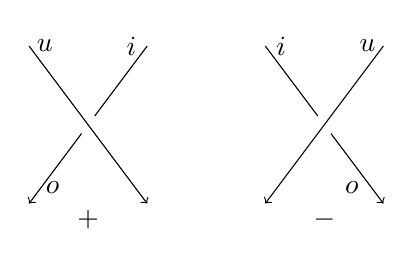
\begin{tikzpicture}
    \draw[<-] (0, -2)--(1.5, 0);
    \fill[white] (0.75, -1) circle (4pt);
    \draw[->] (0, 0)--(1.5, -2);

    \node at (0.75, -2.2) {$+$};
    \node at (0.2, 0) {$u$};
    \node at (1.3, 0) {$i$};
    \node at (0.3, -1.8) {$o$};

    \draw[->] (3, 0)--(4.5, -2);
    \fill[white] (3.75, -1) circle (4pt);
    \draw[<-] (3, -2)--(4.5, 0);
    
    \node at (3.75, -2.2) {$-$};
    \node at (3.2, 0) {$i$};
    \node at (4.3, 0) {$u$};
    \node at (4.1, -1.8) {$o$};
  \end{tikzpicture}
  \caption{\label{fig:4:two:types:crossings}Two types of crossings in oriented knot diagram.}
\end{figure}

Just as before, elements from $M^s$ that map to the trivial element in $M^x$ are responsible for coloring of the diagram being examined.

{\color{yellow}Those two definitions of homomorphism can be used to define two operators $M\times M\to M\times M$ which take segments that enter a crossing and return segments that leave said crossing. Looking from top to bottom of \cref{fig:4:two:types:crossings}, said operators are represented by matrices:}

Those two definitions of homomorphism can be used to define two operators $M\times M\to M\times M$ act on braids by taking strings that go into a crossing and returning those that leave the crossing. Looking from top to bottom of \cref{fig:4:two:types:crossings}, said operators are represented by matrices:
$$
A_+=\begin{pmatrix}
  -c^{-1}a & -c^{-1}b \\
  1 & 0
\end{pmatrix}
\begin{pmatrix}u\\i\end{pmatrix}
\quad\quad\quad
A_-=\begin{pmatrix}
  0 & 1 \\ 
  -\gamma^{-1}\beta & -\gamma^{-1}\alpha
\end{pmatrix}
\begin{pmatrix}i\\u\end{pmatrix}
$$

Considering the braid diagram in \cref{fig:5:first:braid:relation} we can see that given two strings, if we first arrange them in crossing $+$ from \cref{fig:4:two:types:crossings} and immediately after in crossing $-$ we can use Reidemeister's move to obtain identity on those two strands. Thus, we get equality
\begin{align*}
  A_+A_-&=\begin{pmatrix}-c^{-1}a&-c^{-1}b\\ 1 & 0\end{pmatrix}\begin{pmatrix}0&1\\-\gamma^{-1}\beta&-\gamma^{-1}\alpha\end{pmatrix}=\\ 
        &=\begin{pmatrix}c^{-1}b\gamma^{-1}\beta & c^{-1}b\gamma^{-1}\alpha-c^{-1}a\\ 0& 1\end{pmatrix}=Id
\end{align*}
assuming that $c=1=\gamma$ we get
$$b\beta=1$$
$$b\alpha-a=0$$
From the first equality we know that both $b$ and $\beta$ are units in ring $R=\Z[t, t^{-1}]$, therefore we can set $b=t=\beta$.
\begin{figure}[h]\centering 
  \begin{tikzpicture} 
    %\draw (1, 0) to[out=-90, in=90] (1, -1) to [out=225, in=45] (0, -2);
  \pic[
braid/.cd,
every strand/.style={thick},
strand 1/.style={red},
strand 2/.style={green},
gap=.2,
height=1.3cm
] {braid={s_1 s_1^{-1}}};
%\node at (0, 4.8) {$\color{red}x$};
%\node at (1, 4.8) {$\color{green}y$};
\draw[thick, red, ->] (0, 0.1)--(0, 0);
\draw[thick, green, ->] (1, 0.1)--(1, 0);
\draw[thick, red, ->] (3, 3.1)--(3, 0);
\draw[thick, green, ->] (4, 3.1)--(4, 0);
  \end{tikzpicture}
  \caption{\label{fig:5:first:braid:relation}Braid diagram.}
\end{figure}

Using another Reidemeister move as seen in \cref{fig:6:second:braid:relation} we get
$$(a^2+ba+a)x=(ba-ab)y$$
and because $x$ and $y$ are independent strings, both brackets must equal $0$. Thus we arrive at
$$ba=ab$$
$$a(a+b)=-a$$

{\color{red}CZY DODAWAĆ TUTAJ JAK SIĘ TO LICZY TAK PRZEJŚCIE PO PRZEJŚCIU?}

\begin{figure}[h]\centering 
  \begin{tikzpicture}[bbstyle/.style={rectangle, draw=white, fill=white, fill opacity=0.7, text opacity=1, inner sep=2pt}]
    %\draw (1, 0) to[out=-90, in=90] (1, -1) to [out=225, in=45] (0, -2);

\begin{pgfonlayer}{bg}    % select the background layer
        %\draw (0,0) -- (0,2);
  \pic[
braid/.cd,
every strand/.style={thick},
strand 1/.style={red},
strand 2/.style={green},
gap=.2,
height=1.3cm,
width=1.5cm
] {braid={s_1^{-1} s_2^{-1} s_1^{-1} }};
\draw[thick, red, ->] (0, 0.1)--(0,0);
\draw[thick, green, ->] (1.5, 0.1)--(1.5, 0);
\draw[thick, ->] (3, 0.1)--(3, 0);

\node at (0, 4.6) {$x$};
\node at (1.3, 4.6) {$\color{green}y$};
\node at (2.8, 4.6) {$\color{red}z$};

\node[anchor=north west] at (-0.2, 0) {\rotatebox{-30}{$\scriptstyle\color{red}a^2x+aby+bax+b^2z$}};
\node[anchor=north west] at (1.3, 0) {\rotatebox{-30}{$\scriptstyle\color{green}-ax-by$}};
\node[anchor=north west] at (2.8, 0) {\rotatebox{-30}{$\scriptstyle x$}};

  \node[bbstyle, rotate=-30] at (0, 3) {{$\color{green}\scriptstyle-ax-by$}};
  \node[bbstyle, rotate=-30] at (1.5, 3) {{$\scriptstyle x$}};
  \node[bbstyle, rotate=-30] at (3, 1.5) {{$\scriptstyle x$}};
  \node[bbstyle, rotate=-30] at (1.5, 1.5) {{$\color{red}\scriptstyle -ax-bz$}};
\end{pgfonlayer}

\begin{scope}[shift={(4.5, 0)}]
\begin{pgfonlayer}{bg}    % select the background layer
        %\draw (0,0) -- (0,2);
  \pic[
braid/.cd,
every strand/.style={thick},
strand 1/.style={red},
strand 2/.style={green},
gap=.2,
height=1.3cm,
width=1.5cm
] {braid={s_2^{-1} s_1^{-1}  s_2^{-1} }};
\draw[thick, red, ->] (0, 0.1)--(0,0);
\draw[thick, green, ->] (1.5, 0.1)--(1.5, 0);
\draw[thick, ->] (3, 0.1)--(3, 0);

\node at (0, 4.6) {$x$};
\node at (1.3, 4.6) {$\color{green}y$};
\node at (2.8, 4.6) {$\color{red}z$};

\node[anchor=north west] at (-0.2, 0) {\rotatebox{-30}{$\scriptstyle\color{red}a^2x+aby+bax+b^2z$}};
\node[anchor=north west] at (1.3, 0) {\rotatebox{-30}{$\scriptstyle\color{green}-ax-by$}};
\node[anchor=north west] at (2.8, 0) {\rotatebox{-30}{$\scriptstyle x$}};

  \node[bbstyle, rotate=-30] at (3, 3) {{$\color{green}\scriptstyle y$}};
  \node[bbstyle, rotate=-30] at (1.5, 3) {{$\scriptstyle\color{red} -ay-bz$}};
  %\node[bbstyle, rotate=-30] at (0, 1.5) {{$\scriptstyle x$}};
  \node[bbstyle, rotate=-30] at (1.5, 1.5) {{$\scriptstyle x$}};
\end{pgfonlayer}
\end{scope}
  \end{tikzpicture}
  \caption{\label{fig:6:second:braid:relation}Braid diagram.}
\end{figure}
